\subsection{Use Case: Continuous Monitoring for Enterprise Security}


\paragraph*{Background.}
Most modern day big corporations have a hybrid multi-cloud architecture 
with points of presence on-premise and multiple cloud vendors. 
Secure-by-design is a key architectural consideration for these 
enterprises as a safeguard against organized cyber crime activities 
such as ransomware and sensitive data exfiltration. Continuous monitoring 
is one of the key elements for secure-by-design whereby critical 
assets and network communication are continuously monitored for signs 
of suspicious behaviour and any threats identified are responded to in an automated way.

\begin{figure}[htb]
\centering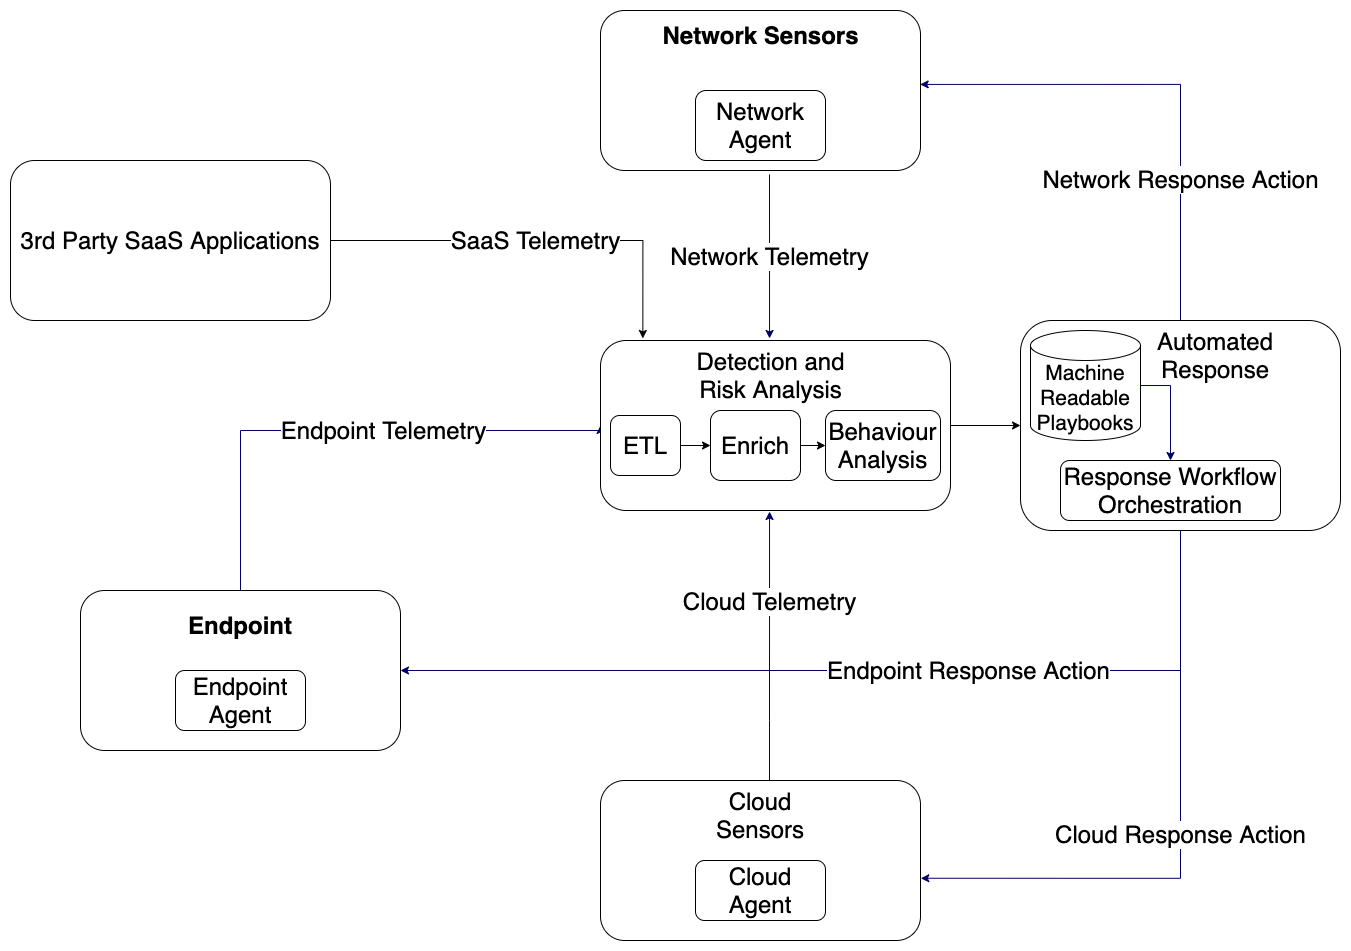
\includegraphics[width=0.8\columnwidth]{usecase/security_usecase_analytics_as_a_service_framework.drawio.png}
\caption{Continuous Monitoring and Response}
\label{fig:sec-general}
\end{figure}

Figure \ref{fig:sec-general} shows a simplified version of a typical 
Continuous Monitoring Pipeline which usually consists of distributed services for the following functions:

\begin{enumerate}

\item{\bf Telemetry Collection.} Telemetry is typically collected from endpoint, 
network, cloud, and 3$^{rd}$-party Software as a Service (SaaS) applications by endpoint, network, and cloud agents, 
firewalls, Web Application Firewall (WAF), email security, and vulnerability scanners. Telemetry usually consists 
of operating system (OS) and application audit logs, vulnerability scan results, oftware Bill Of Materials (SBOMs), east-west and 
north-south network packets and flow logs, cloud policies etc.

\item{\bf Detection and Risk Analysis.} The Detection and Risk Analysis pipeline 
comprises  extract, transform, and load (ETL) for data normalization, enrichment on normalized data by correlating 
with threat intel from inhouse and 3$^{rd}$ party services, and asset profiling and
behavioural analysis for misbehaviour detection which is done using rule-based 
and machine-learning based approaches.

\item{\bf Automated Response.} Automated Response consists of security response 
playbooks and workflows for alerting, breach containment, mitigation, remediation 
and asset recovery.

\end{enumerate}

This use case has the implicit requirements needing the following
aspects to be addressed by the framework we develop.

\begin{enumerate}

\item{\bf AS vendor neutral cloud and computer service integration.}

  \begin{enumerate}
  
  \item {\bf AS in cloud.} The Analytics Service for this use case is typically hybrid with points of presence on premise where analytics modules can run on the sensors and on cloud. On premise sensors can have support for local storage and running light-weight ETL and machine learning inference, whereas cloud can have more heavy-weight compute and machine learning model training and inference support.
  
  \item {\bf AS in LCCF.} This feature does not apply to the current use case.
  
  \item {\bf AS in microservices.} Microservices approach is highly applicable to the design of continuous monitoring pipeline where each of the subfunctions for telemetry collection, ETL, enrichment, analytics and automated response can consist of several microservices that could either be developed in-house or leverage 3rd party SaaS.
  
  \end{enumerate}

\item{\bf AS architecture.}

  \begin{enumerate}
  
  \item{\bf AS vendor neutral interfaces.} Vendor neutral interfaces would be ideal for different functions of the Continuous Monitoring Pipeline. However, at this time there are no standardized interfaces for technologies related to continuous monitoring. Each vendor typically has its own proprietary set of interfaces and data models and it is upto the consumer of the data to normalize that data.
  
  \item{\bf AS REST.} REST is typically used for human and M2M interfaces at different levels in the Continuous Monitoring pipeline. On-premise and cloud agents for telemetry collection support both data push and pull via REST interface. Data Enrichment services can be in-house and 3rd party SaaS which typically have REST interfaces for pulling reference datasets. Analytics and Automated Response pipelines typically have REST interfaces for pipeline configuration and adding or updating content.
  
  \item{\bf AS layers such as interface, service layer, and provider layer.} Interface layer is required for data access for experimentation and use case development, for configuring and adding new functions and content to telemetry collection, analytics and response functions. Service layer is required to register in-house and 3rd party microservices to support the continuous monitoring pipeline and to register analytics workflows. Provider layer is required to schedule services and workflows on-premise and on cloud.
  \end{enumerate}

\item{\bf AS workflow.}

  \begin{enumerate}
  
  \item{\bf AS catalog and registry.} Continuous Monitoring will comprise several microservices for telemetry collection, ETL, enrichment, analytics, and automated response. These services can be in-house or 3rd party SaaS services running remotely and accessible via APIs. The catalog and registry functionality will be required to catalog and register these services and have required configuration for service setup and service access.
  
  \item{\bf AS cooperation.} There can be intra and inter-function collaboration between the services that are part of the Continuous Monitoring Pipeline. For instance, endpoint, network and cloud agents belong to the telemetry collection function and can have intra-function collaboration where they can cooperate with one another on what telemetry to collect on the fly based on contextual and situational awareness. There is also inter-function collaboration for instance between automated response pipeline and endpoint, network and cloud agents for breach containment, mitigation and asset recovery.
  
  \item{\bf AS competition.} There can also be competing services and rules can be defined on how to orchestrate between these competing services. For instance for instance the Continuous Monitoring Pipeline can have multiple 3rd party and in-house services for threat intel enrichment and rulessets can be defined on how to orchestrate between these services to streamline cost, speed, and resources.
  
  \item{\bf AS orchestrator.} API-based workflow definition, and orchestration capabilities are required for the Continuous Monitoring Pipeline to orchestrate cooperating functions and cooperating and competing microservices that are part of those functions.
  
  \end{enumerate}


\item{\bf AS calculation.}

  \begin{enumerate}
  
  \item{\bf AS with DL.} Deep Learning is leveraged in the analytics stack for behaviour profiling and misbehaviour detection and knowledge graph analysis (e.g., graph neural networks and neuro symbolic analysis).
  
  \item{\bf AS data analytics.} Data analytics is leveraged for data visualization and model quality and drift detection, and visualizing and report generation on security outcomes and alerts. 
  
  \end{enumerate}

\item{\bf AS security.} AS Security is required for securing data at rest and during transit, for securely storing service access credentials, and for enforcing resource access and usage policies. 

\end{enumerate}


